\documentclass[12pt,twoside]{article}
    \usepackage{jmlda}
    \usepackage{graphics}
    \usepackage{booktabs}
    \usepackage{wrapfig}
    \usepackage{multirow}
    \usepackage{enumitem}
    \setcounter{secnumdepth}{3}

    %\NOREVIEWERNOTES
    \title
        {Динамическое выравнивание многомерных временных рядов}
    \author
        {Гончаров~А.\,В., Моргачев~Г.\,И., Смирнов~В.\,, Липницкая~Т.\,} % основной список авторов, выводимый в оглавление
    \thanks{
        Работа выполнена при финансовой поддержке РФФИ, проект \No\,00-00-00000.
        Научный руководитель:  Гончаров~А.\,В.
        Задачу поставил:  Гончаров~А.\,В.
        Консультант:  Гончаров~А.\,В.
    }
    \email
        {morgachev.gi@phystech.edu, smirnov.vs@phystech.edu, tanya.lipnizky@yandex.ru}
    \organization
        {МФТИ}

    \abstract{
        В работе исследуется зависимость качества решения задач метрической кластеризации и метрического поиска эталонной подпоследовательности для многомерных временных рядов от выбранной функции расстояния между объектами.
        Базовая фукнция расстояния между временными рядами основана на методе динамического выравнивания оси времени. Однако в базовой реализации алгоритм применим лишь к случаю одномерного временного ряда. 
        Работа предлагает модификацию оптимизированного алгоритма расчета функции расстояния между объектами, основанного на динамическом выравнивании оси времени. 
        Для анализа зависимости качества решения поставленных задач выбраны несколько модификаций базовой функции расстояния. 
        Результаты моделирования представлены в работе на основе размеченных данных о деятельности человека полученных с носимого устройства.
        Обоснованность метрического подхода к решению задачи демонстрируется путем сравнения с результатами на основе авторегрессионной модели. 

        \bigskip
        \textbf{Ключевые слова}: \emph {временные ряды, многомерные временные ряды, DTW}.
    }
    
    % \titleEng
    %     {JMLDA paper example: file jmlda-example.tex}
    % \authorEng
    %     {Author~F.\,S.$^1$, CoAuthor~F.\,S.$^2$, Name~F.\,S.$^2$}
    % \organizationEng
    %     {$^1$Organization; $^2$Organization}
    % \abstractEng
    %     {This document is an example of paper prepared with \LaTeXe\
    %     typesetting system and style file \texttt{jmlda.sty}.
    
    %     \bigskip
    %     \textbf{Keywords}: \emph{keyword, keyword, more keywords}.}
        
    \begin{document}

    \maketitle
    \setcounter{secnumdepth}{3}
    \section{Введение}\label{intro}
        
        Для описания различных данных широко используются временные ряды.
        Чтобы найти их сходство вводится функция расстояния, однако стандартный поточечный подход не является информативным вследствие того,
        что ряды могут содержать общие паттерны, деформированные относительно временной оси: претерпевшие сдвиги либо сжатия \cite{01f4ab11a9ff49ff909094a135dcfe33}.
        Одним из способов решения этой проблемы является выравнивание временных рядов (DTW)  \cite{Keogh01derivativedynamic} и его модификаций \cite{journals/ida/SalvadorC07}.
        Этот подход в большом спектре задач позволяет достичь максимального качества среди его аналогов.
        
        В работе рассматривается применения DTW для кластеризации рядов и поиска подпоследовательностей
        соответствующих некоторому классу событий для случая многомерных рядов.
        Использование DTW на подобных данных описано в \cite{Holt2007,Sanguansat2012MultipleMS}.
        В работе \cite{Holt2007} предлагается способ выравнивания многомерных рядов, основанный на нормализации исходных данных и нахождении векторной нормы.
        В \cite{Sanguansat2012MultipleMS} рассматривается алгоритм, позволяющий выполнить выравнивание временных рядов между координатами. 
        Многомерное DTW предполагает различные варианты выравнивания, такие как выравнивание относительно общей временной шкалы и между соответсвующими каналами.
        
        В процессе работы алгоритма DTW происходит вычисление расстояний между точками сравниваемых рядов.
        Поскольку в многомерном случае координаты точек описываются векторами, на результат будет влиять выбор функций расстояния между ними.
        Исследование влияние выбора этих функций на качество кластеризации является главной особенностью этой работы.
        В работе используются функции расстояния порождённые $L_1$ и $L_2$ нормами.
        
        Ещё одним стандартным подходом к нахождению сходства между рядами является сравнение представления рядов коэффициентами их регрессионных моделей.
        Полученная в ходе работы DTW кластеризация сравнивается с кластеризацией на основе авторегрессионной модели.
    
        % вставить обзор методов из статьи! 
        В статьях \cite{WARRENLIAO20051857} \cite{AGHABOZORGI201516} рассматриваются различные виды алгоритмов кластеризации временных рядов,
        среди которых неплохие результаты показывают варианты иерархической кластеризации.
        Данный вид кластеризации был выбран в качестве базового.
        
		% проапдейтить инфу о данных 
        Данные \cite{Kwapisz:2011:ARU:1964897.1964918} представляют собой измерения акселерометра некоторого носимого устройства,
        например мобильного телефона, находящегося в кармане человека, и используется для индентификации действия человека в конкретный момент времени.
        Данные разделены на 6 классов: ходьба, бег, подъём по лестнице, спуск по лестнице, сидение, лежание.
        
        
    \section{Постановка задачи}\label{problem}
		
        Временнным рядом называется упорядоченная последовательность измерений\\
        $S = s_1,s_2,...,s_n$,
        где $n$ \-- длина временного ряда.
        
        Поскольку мы используем многомерные временные ряды, то $s_i, i \in 1\dots n$, представляют собой вектор размерности $l$.
        Например, при рассмотрении задачи идентификации определенного движения человека вектор является трёхмерным с координатами $(x, y, z)$.

        Имеется множество функций расстояния между векторами $\boldsymbol{R}$:
        $$
            \boldsymbol{R} = \{\rho: \mathbb{R}^l \times \mathbb{R}^l \rightarrow \mathbb{R}_+ \}
        $$
				
        Каждой функции расстояния $\rho$ между векторами соответствует функция расстояния между временными рядами:
        $$\text{DTW}_{\rho}: \boldsymbol{S} \times \boldsymbol{S} \rightarrow \mathbb{R}_+.$$

        Целью эксперимента является изучения влияния выбора поточечной метрики на результат работы DTW на примере двух задач,
            описанных в разделе 3:
    
        \begin{enumerate}[label=\arabic*)]
            \item Поиск шаблонов в ряду
            \item Кластеризация рядов
        \end{enumerate}        
                
        Для данных задач задаются соответствующие метрики качества $Q_i$.
        Тогда, решаемая задача определения оптимальной метрики:
        $$
            \rho_i^* = \argmax_\rho Q_i(\rho)
        $$

        Рассматриваются следующие функций расстояния между векторами:         
        \begin{enumerate}[label=\arabic*)]
            \item $L_1(v, u) = {\displaystyle\sum_{l = 1}^{l} |v_i - u_i|}$
            \item $L_2(v, u) = \sqrt{\displaystyle\sum_{l = 1}^{l} (v_i - u_i)^2}$,
                евклидово расстояние, также будем обозначать его $ED(u, v)$
            \item $\text{cosine}(v, u) = 1 - \dfrac{(v, u)}{\sqrt{(v, v)}\sqrt{(u, u)}}$
        \end{enumerate}

        Кроме того, производится сравнения качества и скорости работы данного подхода с другими используемыми методами:
        \begin{enumerate}[label=\arabic*)]
            \item Функция расстояния на основе поточечных расстояний между рядами, при равным длинах рядов:
                $$
                    ED(S_1, S_2) = \sum\limits_1^m \|s_{1i} - s_{2i}\|_2
                $$

            \item Применение авторегрессионной модели для описания ряда.
        \end{enumerate}
    
    \section{Рассматриваемые задачи}\label{tasks}
        \paragraph{Поиск паттернов}
        
        Рассматривается задача поиска заранее известных паттернов во временном ряду. 
        Имеется временной ряд $S$ длинны $n$, содержащий сегменты класса $\boldsymbol{P}$.
        Класс $\boldsymbol{P}$ \-- в нашем случае, набор временных рядов длины $m \ll n$. \\
        Известо $k$ представителей класса $\boldsymbol{P}$, \textit{не содержащихся в $S$}. \\
        Необходимо найти участки $S$, соответствующие данному классу. \\
        Обозначим множество начал таких участков как $\boldsymbol{T} = \{t_1, \dots, t_j \}$.

        Будем считать участок найденным, если его пересечение с предполагаемым участком более $80\%$ длины $m$.
        Поиск будет проводиться путем нахождения расстояния с помощью $DTW_{\rho}$ между фрагментами ряда $S$ и шаблоном,
            полученным из известных экземпляров класса. 

        Рассматриваемая функция качества:
        \begin{align*}
            Q_3(DTW_{\rho}) = \dfrac{\sum\limits_{i=1}^j [t_i \-- \text{найден}]}{j}.
        \end{align*}

        \paragraph{Кластеризация}
        Исходные данные представляют собой временные ряды (длиной n).
        Имеется выборка $ S \subset \mathbb{S}$ из $N$ элементов.
        Для каждого элемента выборки $s_i$ известна метка класса $y_i \in \mathbb{Y}$, где $\mathbb{Y}$
            \-- множество меток классов.

        Определим матрицу попарных расстояния:
        $$D(\text{DTW}_\rho(\boldsymbol{S})) = ||D_{ij}||, \ \ D_{ij} = \text{DTW}_\rho(S_i, S_j),\ \ S_i, S_j \in \boldsymbol{S}.$$
        И модель кластеризации:
        $$
            f: D \rightarrow Z^N
        $$

        Где $Z$ \-- множество меток кластеров.
        Будем рассматривать следующие функции качества:
        \begin{align*}
            Q_1(f(D), S) &= \frac{1}{|Z|}\sum\limits_{z \in Z} \max_y \frac{N_z^y}{N_z}  \\
            Q_2(f(D), S) &= \frac{1}{|Z|}\sum\limits_{z \in Z} \max_y \frac{(N_z^y)^2}{N_z N^y}
            % Q(f(D), S) = \frac{\sum\limits_{s_i, s_j \in S} \mathbb{I}(z_i = z_j \land  y_i = y_j)}{N^2}            
        \end{align*}
        Здесь: 
        \begin{itemize}[label=$\bullet$]
            \item $N_z$ \-- количество элементов в кластере с меткой $z$. 
            \item $N^y$ \-- количество элементов в классе $y$.
            \item $N_z^y$ \-- количество элементов класса $y$ в классе $z$.
        \end{itemize}

        % Пусть $s_i \in \mathbb{R}^n $ - временные ряды, являющиеся объектами некоторой выборки,
        % $\rho$ - некоторые выбранные метрики, $Q$ - критерий качества (данные с соизмеримым количеством точек), являющийся ответом.
        % Требуется постороить такую функцию выравнивания, что:
        % $ f = argmin(Q(s_i, \rho))$
                
    \section{Описание основных методов}
        
        Для построения функции выравнивания и проверки её качества используются модель DTW (и её отптимазации).
            
    \paragraph{Описание функции расстояния между объектами}

        В данной работе в качестве метрического расстояния между объектами предлагается использовать строимость
        \textit{пути наименьшей стоимости} между объектами.
            
        Dynamic time warping - измерение расстояния между двумя временными рядами.
            
        Задано два временных ряда, $X$ длины $m_1$ и $Y$ длины $m_1$.
            \begin{align*}
                X &= x_1,x_2, ..., x_i, ..., x_{m_1} \\
                Y &= y_1,y_2, ..., y_j, ..., y_{m_2} \\
                & x_i, y_j \in \mathbb{R}^n
            \end{align*}

        Требуется построить матрицу размера $m_1\times m_2$ c элементами $D_{ij}=d(x_i, y_j)$, где d - выбранная метрика.
            
        Чтобы найти наибольшее соответствие между рядами нужно найти выравнивающий путь W, который минимизирует расстояние между ними.
        W - набор смежных элементов матрицы D, $w_k = (i, j)_k$.
            
            $W = w_1,w_2, ..., w_k, ..., w_K $

            $max(m_1, m_2)\leq K \leq m_1 + m_2 + 1$, где K-длина выравнивающего пути
            
        Выравнивающий путь должен удовлетворять следующим условиям:
            \begin{enumerate}[label=\arabic*)]
                \item $w_1=(1,1)$, $w_K=(m_1, m_2)$
                \item $w_k = (a, b)$, $w_{k-1}=(a', b')$ : $a-a' \leq 1$, $b-b' \leq 1$ 
                \item $w_k = (a, b)$, $w_{k-1}=(a', b')$ : $a-a' \geq 0$, $b-b'\geq 0$
            \end{enumerate}

        Оптимальный выравнивающий путь должен минимизировать выравнивающую стоимость пути:
            $$
                DTW(X, Y)=\displaystyle\sum\limits_{k=1}^{K} w_k
            $$
            
        Путь находится рекуррентно:\\
            $\gamma(i, j) = d(q_i, c_j) + min({\gamma(i-1, j-1), \gamma(i-1, j), \gamma(i, j-1)})$ ,
            где $\gamma(i, j)$ суммарное расстояние, $d(q_i, c_j)$ расстояние в текущей клетке.
						
                Кроме того, выравнивающий путь ограничивают тем, насколько он может отклоняться от диагонали.
                Типичным ограничением является полоса Сако-Чиба, накладывающая условие, что путь искривления не может отклоняться от диагонали больше,
                чем на определённый процент клеток.

	\paragraph{Описание алгоритма кластеризации}      
        В качестве алгоритма кластеризации используется иерархическая кластеризация, которая базируется на последовательном слияние ближайших кластеров.
        Рассматриваются различные функции расстояния между кластерами: 
        \begin{enumerate}
            \item \textit{complete:}  $d(A, B) = \max\limits_{a \in A, b \in B}(dist(a, b))$ 
            \item \textit{weighted:}  $d(A,B) = \dfrac{(dist(S,B) + dist(T,B))}{2}$, где кластер $A = S \cup T$
            \item \textit{average:}   $d(A,B) = \sum\limits_{a \in A, b \in B} \dfrac{d(a, b)}{(|A|*|B|)}$ 
        \end{enumerate} 
                
    % TODO: formal check it
    \section{Оптимизации}
        В основу нашей реализации легла работа \cite{Rakthanmanon:2012:SMT:2339530.2339576}, в которой было
        использовано большое количество оптимизаций, позволяющих как сократить время вычисления расстояния 
        между рядами, так и, при возможности, вообще не вычислять его. 
        В ходе работы мы постарались обобщить эти оптимизации на многомерный случай.
        Ниже приведено их краткое описание. 

        \paragraph{Использование квадрата расстояния}	
        В DTW вычисляется квадратный корень, однако, если упустить этот шаг,
        относительное расстояние не изменится, поскольку обе функции монотонны и вогнуты.
        Это упрощает вычисления и позволяет сделать модель легкой для понимания.
        Таким образом, говоря о DTW, мы подразумеваем квадратные аналоги.
        
        \paragraph{Использование нижней границы}
        Для того чтобы ускорить последовательный поиск в DTW, используется нижняя граница (Lower Bounding),
        чтобы отбросить неподходящие последовательности (подпоследовательности).
        Оптимизация ускоряет поиск ещё и потому что не требует затратных вычислений.
        
        В эксперименте используется каскадная нижняя граница.
        Вначале последовательность проходит проверку на требования $LB_{Kim}$,
        которая использует расстояние между максимальными значениями рядов и минимальными значениями рядов.
        Однако, для того чтобы сравнить последовательности, они должны быть нормализованы,
        поэтому значения двух расстояний между максимальными и минимальными точками могут быть ничтожно малы.
        В случае если последовательность удовлетворила требованиям $LB_{Kim}$, происходит вторичная проверка $LB_{Keogh}$, использующей ED.
        
        Также бывает полезным менять роли сравниваемых последовательностей для $LB_{Keogh}$,
        от этого будет меняться решение к какой последовательности применяется нижняя граница,
        причем результаты вычисления этих границ для каждой из последовательностей при их сравнении в общем случае не будут равны.
        Однако данный метод применяется опционально и только в том случае, если другие нижние границы не проявили себя.
        
        \paragraph{Использование верхней границы}
        При вычислении $LB_{Keogh}$, мы можем заметить,
        что текущая сумма расстояний между каждой парой точек привысила определённое (наибольшее возможное) значение,
        в таком случае мы можем прекратить подсчёт, тк дальнейший действия дадут ещё более высокий результат.
        
        Если вся $LB_{Keogh}$ была посчитана и мы обнаружили, что должны вычислить DTW полностью,
        есть способ отбросить лишние вычислительные затраты на стадии подсчёта DTW.
        Если постепенно вычислять DTW слева направо от 1 до k и суммировать частичное накопление DTW с вкладом от $LB_{Keogh}$ от k+1 до n.
        Сумма $DTW(S_{1:k}^i, S_{1:k}^j) + LB_{Keogh}(S_{k+1:n}^i, S_{k+1:n}^j)$ является нижней границей для $DTW(S_{1:n}^i, S_{1:n}^j)$.
        Если в какой-то момент такая нижняя граница превысит верхнюю, расчёт прекращается.
        Кроме того, расходы на расчёт такой границы незначительны.
        
        % Мы не переделали программу для ED, напишу на питоне

        % Практически очевидно, что для сравнения двух временных рядов они должны быть нормализованы.
        % Однако она занимает больше времени, чем подсчёт ED. Таким образом было решено объединить ED ($LB_Keogh$) c Z-нормализацией.
        % Постепенно вычисляя нормализацию, мы в той же точке вычисляем ED ($LB_{Keogh}$).
        % Это позволяет отбросить неподходящую последовательность не только на стадии подсчёта дистанции, но и на стадии нормализации.
        
        Во многих случаях становится полезным изменить порядок поиска верхней границы.
        Очевидно, что разный порядок поиска приносит разное ускорение, более того существует n! выриантов упорядочивания.
        Чтобы найти оптимальный вариант, предлагается отсортировать индексы основанных на абсолютных значениях Z-нормализованной последовательности.
        Одно значение временного ряда $S_i$ сравнивается со многими из ряда $S_j$, которые далее сортируются по убыванию вклада ED. 
        % Такая сортировка может быть применена как к $LB_{Keogh}$, так и к отбрасыванию неподходящей последовательности на стадии нормализации.
						
    \section{Эксперимент}

        \paragraph{Нахождение подпоследовательностей}
        Использовалось две выборки, первая из которых состояла из временных рядов длиной в 182 точки с тремя каналами, соответсвующих координатам $X, Y$ 
            и силе нажатия на экран планшета.
        Вторая выборка состояла из временных рядов активности мозга в разных состояниях: эпилепсия, ходьба, бег, просмотр картинок и имеет длину элемента в 206 точек.
        Второй датасет имел многократно меньший размер, но при этом он значительно отличается от первого: периоды повторения паттернов значительно меньше.

        В обеих выборках из каждого класса выбиралось случайное подмножество представителей, из которых,
            путем усреднения методами $DBA$ и простым средним, получались поисковые шаблоны. 
        Путем склейки оставшихся рядов в случайном порядке, создавался длинный ряд, в котором производился поиск $k$ наиболее близких фрагментов 
            для каждого из шаблонов с использованием $ED$ и $DTW_\rho$ с различными $\rho$ в качестве функций расстояния.
            
        Для оценки погрешностей измерений, описанная процедура была проведена с большим количество (20) выборок, полученными из исходной с помощью бутстрепа.    
    
        \begin{table}[h]
            \centering
            \begin{tabular}{c|c *{2}{|*{3}{c}}}  
                \toprule
                  \multirow{2}{*}{$\rho$}& \multirow{2}{*}{average} & 
                            \multicolumn{3}{c|}{characters} & \multicolumn{3}{c}{epi} \\
                \cmidrule(r){3-8}
                                   &  & $Q$ & $t$ & $t_{\text{no optim}}$ & $Q$ & $t$ & $t_{\text{no optim}}$ \\
                \midrule
            \multirow{2}{*}{$L_1$} 
                    & DBA    & $0.83\pm 0.14$ & $2.85\pm 0.43$ & $11\pm 1$ & $0.53\pm 0.10$ & $26\pm 1$ & $25\pm 1$ \\
                    & mean   & $0.87\pm 0.12$ & $2.77\pm 0.45$ & $14\pm 1$ & $0.49\pm 0.08$ & $26\pm 1$ & $28\pm 2$\\
                    
            \midrule\multirow{2}{*}{$L_2$} 
                    & DBA    & $0.80\pm 0.17$ & $2.24\pm 0.30$ & $13\pm 1$ & $0.55\pm 0.07$ & $23\pm 1$ & $26\pm 2$ \\
                    & mean   & $0.84\pm 0.13$ & $2.17\pm 0.22$ & $10\pm 1$ & $0.48\pm 0.10$ & $23\pm 1$ & $26\pm 2$ \\
                    
            \midrule\multirow{2}{*}{$\text{cosine\_dist}$} 
                    & DBA    & $0.77\pm 0.18$ & $3.42\pm 1.00$ & $16\pm 1$ & $0.35\pm 0.10$ & $29\pm 2$ & $38\pm 2$ \\
                    & mean   & $0.81\pm 0.15$ & $3.43\pm 0.83$ & $14\pm 1$ & $0.27\pm 0.06$ & $26\pm 2$ & $38\pm 1$ \\
            \midrule     
            \multirow{2}{*}{ED}
                    & DBA    &   0.08   &   17.511   &    17.511   &    0.172  &   1.620   &    1.620   \\
                    & mean   &   0.09   &   17.645   &    17.645   &    0.172  &   1.540   &    1.540    \\
            \bottomrule
            \end{tabular}
            \caption{Поиск паттернов.}
        \end{table}

        Можно заметить, что на всех данных использование $L_1$ метрики дало лучшие результаты в данной задаче.
        При этом оптимизации позволили сократить время работы в более чем 5 раз на большом датасете (цифры),
            но незначительно в малом, при этом сохранив результаты.

        
        \paragraph{Кластеризация}
        В ходе эксперимента были использованы данные акселерометра мобильного телефона.
        Они представляли собой временные ряды длинной в 600 точек ускорений по осям $X, Y, Z$.
        Из них методом бутстрепа были сгенерированы 20 выборок из 600 рядов по 50 точек в каждом. 
        Каждых из рядов принадлежал к одному из четырёх возможных классов. Данные были равномерно распределены по всем классам.

        Для $DTW$, $ED$ вычислялись матрицы попарных расстояний между парами рядов, на основе которых проводилась кластеризация описанными выше методами.
        В качестве функий расстояния между векторами использовались метрики, порождённые $L_1$  и $L_2$ нормами.
        Кроме того, для каждого из временных рядов была обучена авторегрессионная модель, на основе коэффициентов которых также произведена кластеризация.
        Так как в процессе получения данных были возможны различные положения телефона в кармане, кластеризация проводилась на 4, 12, 24, 36 и 48 кластеров.

        \begin{table}[h]
            \centering
            \begin{tabular}{c|c *{2}{|*{3}{c}}}
                \toprule
                \multirow{2}{*}{$\rho$} & \multirow{2}{*}{$N_{clust}$} & \multicolumn{3}{c|}{$Q_1$} & \multicolumn{3}{c}{$Q_2$} \\
                \cmidrule(r){3-8}
                && \textit{complete} & \textit{average} & \textit{weighted} & \textit{complete} & \textit{average} & \textit{weighted} \\
                \midrule
            \multirow{5}{*}{$L_1$}
                    &  4 & $0.42\pm 0.07$ & $0.51\pm 0.07$ & $0.55\pm 0.06$ & $0.22\pm 0.09$ & $0.31\pm 0.10$ & $0.36\pm 0.09$ \\
                    & 12 & $0.46\pm 0.09$ & $0.54\pm 0.04$ & $0.57\pm 0.04$ & $0.24\pm 0.05$ & $0.33\pm 0.05$ & $0.36\pm 0.05$ \\
                    & 24 & $0.50\pm 0.03$ & $0.57\pm 0.03$ & $0.59\pm 0.03$ & $0.28\pm 0.03$ & $0.36\pm 0.04$ & $0.38\pm 0.04$ \\
                    & 36 & $0.55\pm 0.02$ & $0.60\pm 0.02$ & $0.61\pm 0.03$ & $0.33\pm 0.03$ & $0.40\pm 0.03$ & $0.41\pm 0.05$ \\
                    & 48 & $0.58\pm 0.02$ & $0.63\pm 0.02$ & $0.64\pm 0.03$ & $0.37\pm 0.03$ & $0.43\pm 0.03$ & $0.44\pm 0.04$ \\
            \midrule
            \multirow{5}{*}{$L_2$}
                    &  4 & $0.42\pm 0.06$ & $0.47\pm 0.07$ & $0.54\pm 0.06$ & $0.22\pm 0.07$ & $0.26\pm 0.09$ & $0.35\pm 0.09$\\
                    & 12 & $0.46\pm 0.04$ & $0.53\pm 0.04$ & $0.59\pm 0.04$ & $0.25\pm 0.05$ & $0.32\pm 0.05$ & $0.39\pm 0.05$ \\
                    & 24 & $0.50\pm 0.03$ & $0.57\pm 0.03$ & $0.59\pm 0.03$ & $0.28\pm 0.03$ & $0.35\pm 0.04$ & $0.39\pm 0.03$ \\
                    & 36 & $0.54\pm 0.03$ & $0.60\pm 0.03$ & $0.62\pm 0.03$ & $0.33\pm 0.03$ & $0.40\pm 0.04$ & $0.42\pm 0.03$ \\
                    & 48 & $0.58\pm 0.02$ & $0.63\pm 0.03$ & $0.64\pm 0.03$ & $0.37\pm 0.03$ & $0.43\pm 0.04$ & $0.46\pm 0.04$ \\
            \midrule
            \multirow{5}{*}{$AR$}
                    &  4 & \multicolumn{3}{c|}{$0.52\pm 0.06$} & \multicolumn{3}{c|}{$0.32\pm 0.08$}\\
                    & 12 & \multicolumn{3}{c|}{$0.61\pm 0.05$} & \multicolumn{3}{c|}{$0.42\pm 0.06$} \\
                    & 24 & \multicolumn{3}{c|}{$0.67\pm 0.05$} & \multicolumn{3}{c|}{$0.51\pm 0.07$} \\
                    & 36 & \multicolumn{3}{c|}{$0.70\pm 0.03$} & \multicolumn{3}{c|}{$0.55\pm 0.05$} \\
                    & 48 & \multicolumn{3}{c|}{$0.73\pm 0.03$} & \multicolumn{3}{c|}{$0.59\pm 0.05$} \\
            \bottomrule
            \end{tabular}
            \caption{Кластеризация.}
        \end{table}

    В большинстве случаев лучшие результаты показал метод кластеризации $weighted$.
    При этом, методы выравнивания с $L_1$ и $L_2$ метриками показали примерно равные результаты. Простейшая регрессионная модель позволила достичь лучшего качества во всех экспериментах.
						
    На картинках \ref{img1}, \ref{img2} приводится примеры рядов, отнесенных к одному кластеру,
        выравненных относительно случайного ряда из данного кластера для $L_1$ и $L_2$ метрик соответственно.
    Кластеризация в данных примерах проводилась с помощью метода $weighted$.

    \begin{figure}[h!]
        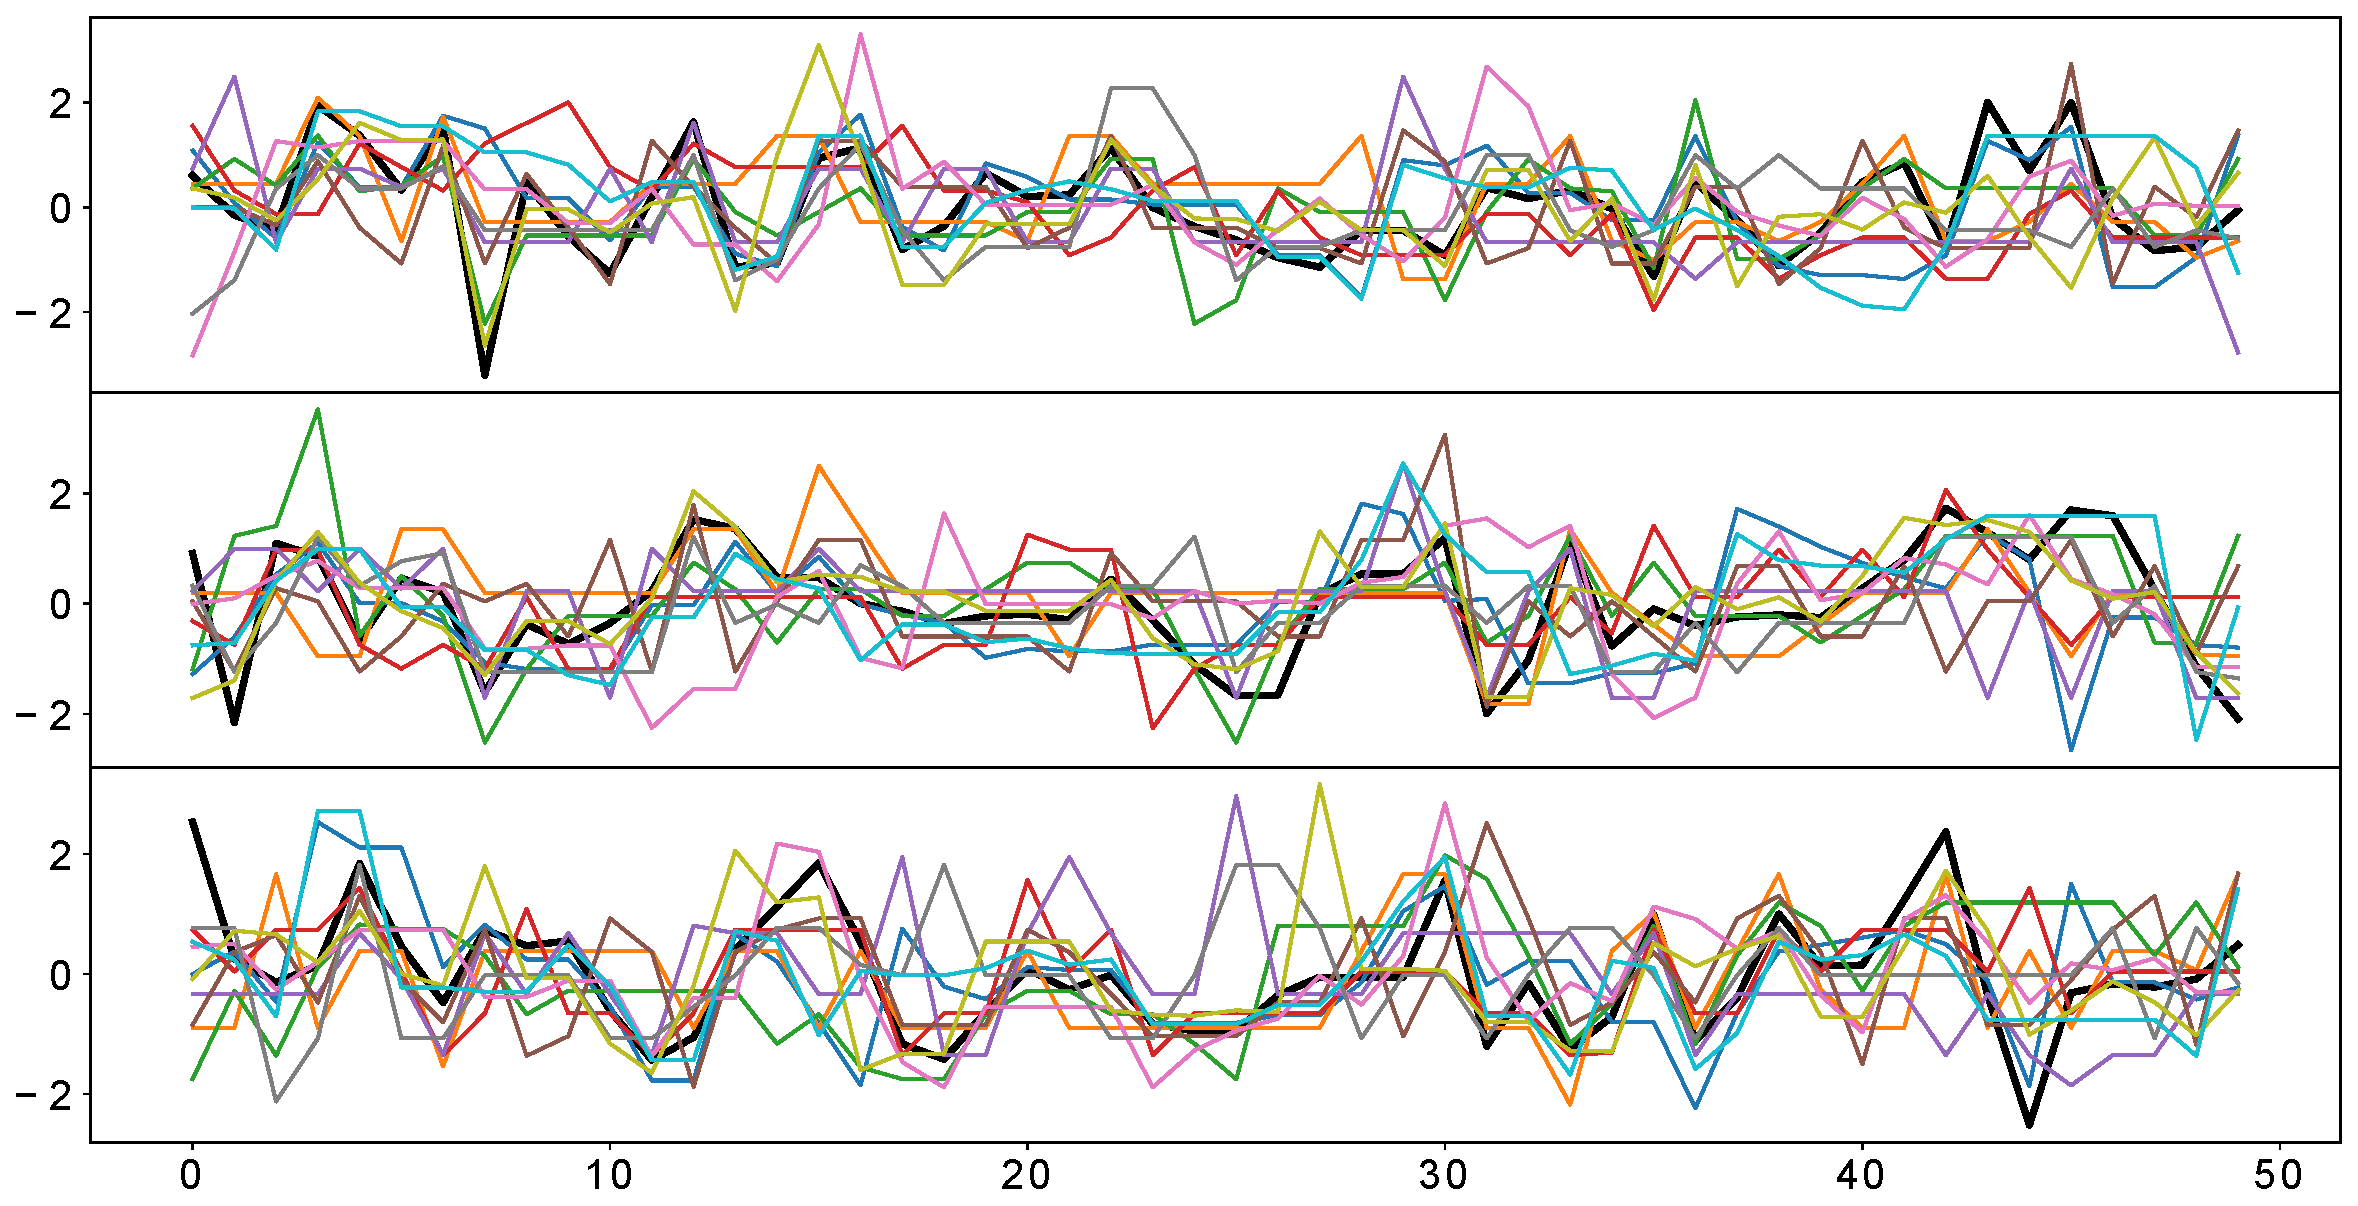
\includegraphics[width=\textwidth]{images/img2.eps}
        \caption{Кластеризация с $L_1$} \label{img1}
    \end{figure}
    \begin{figure}[h!]
        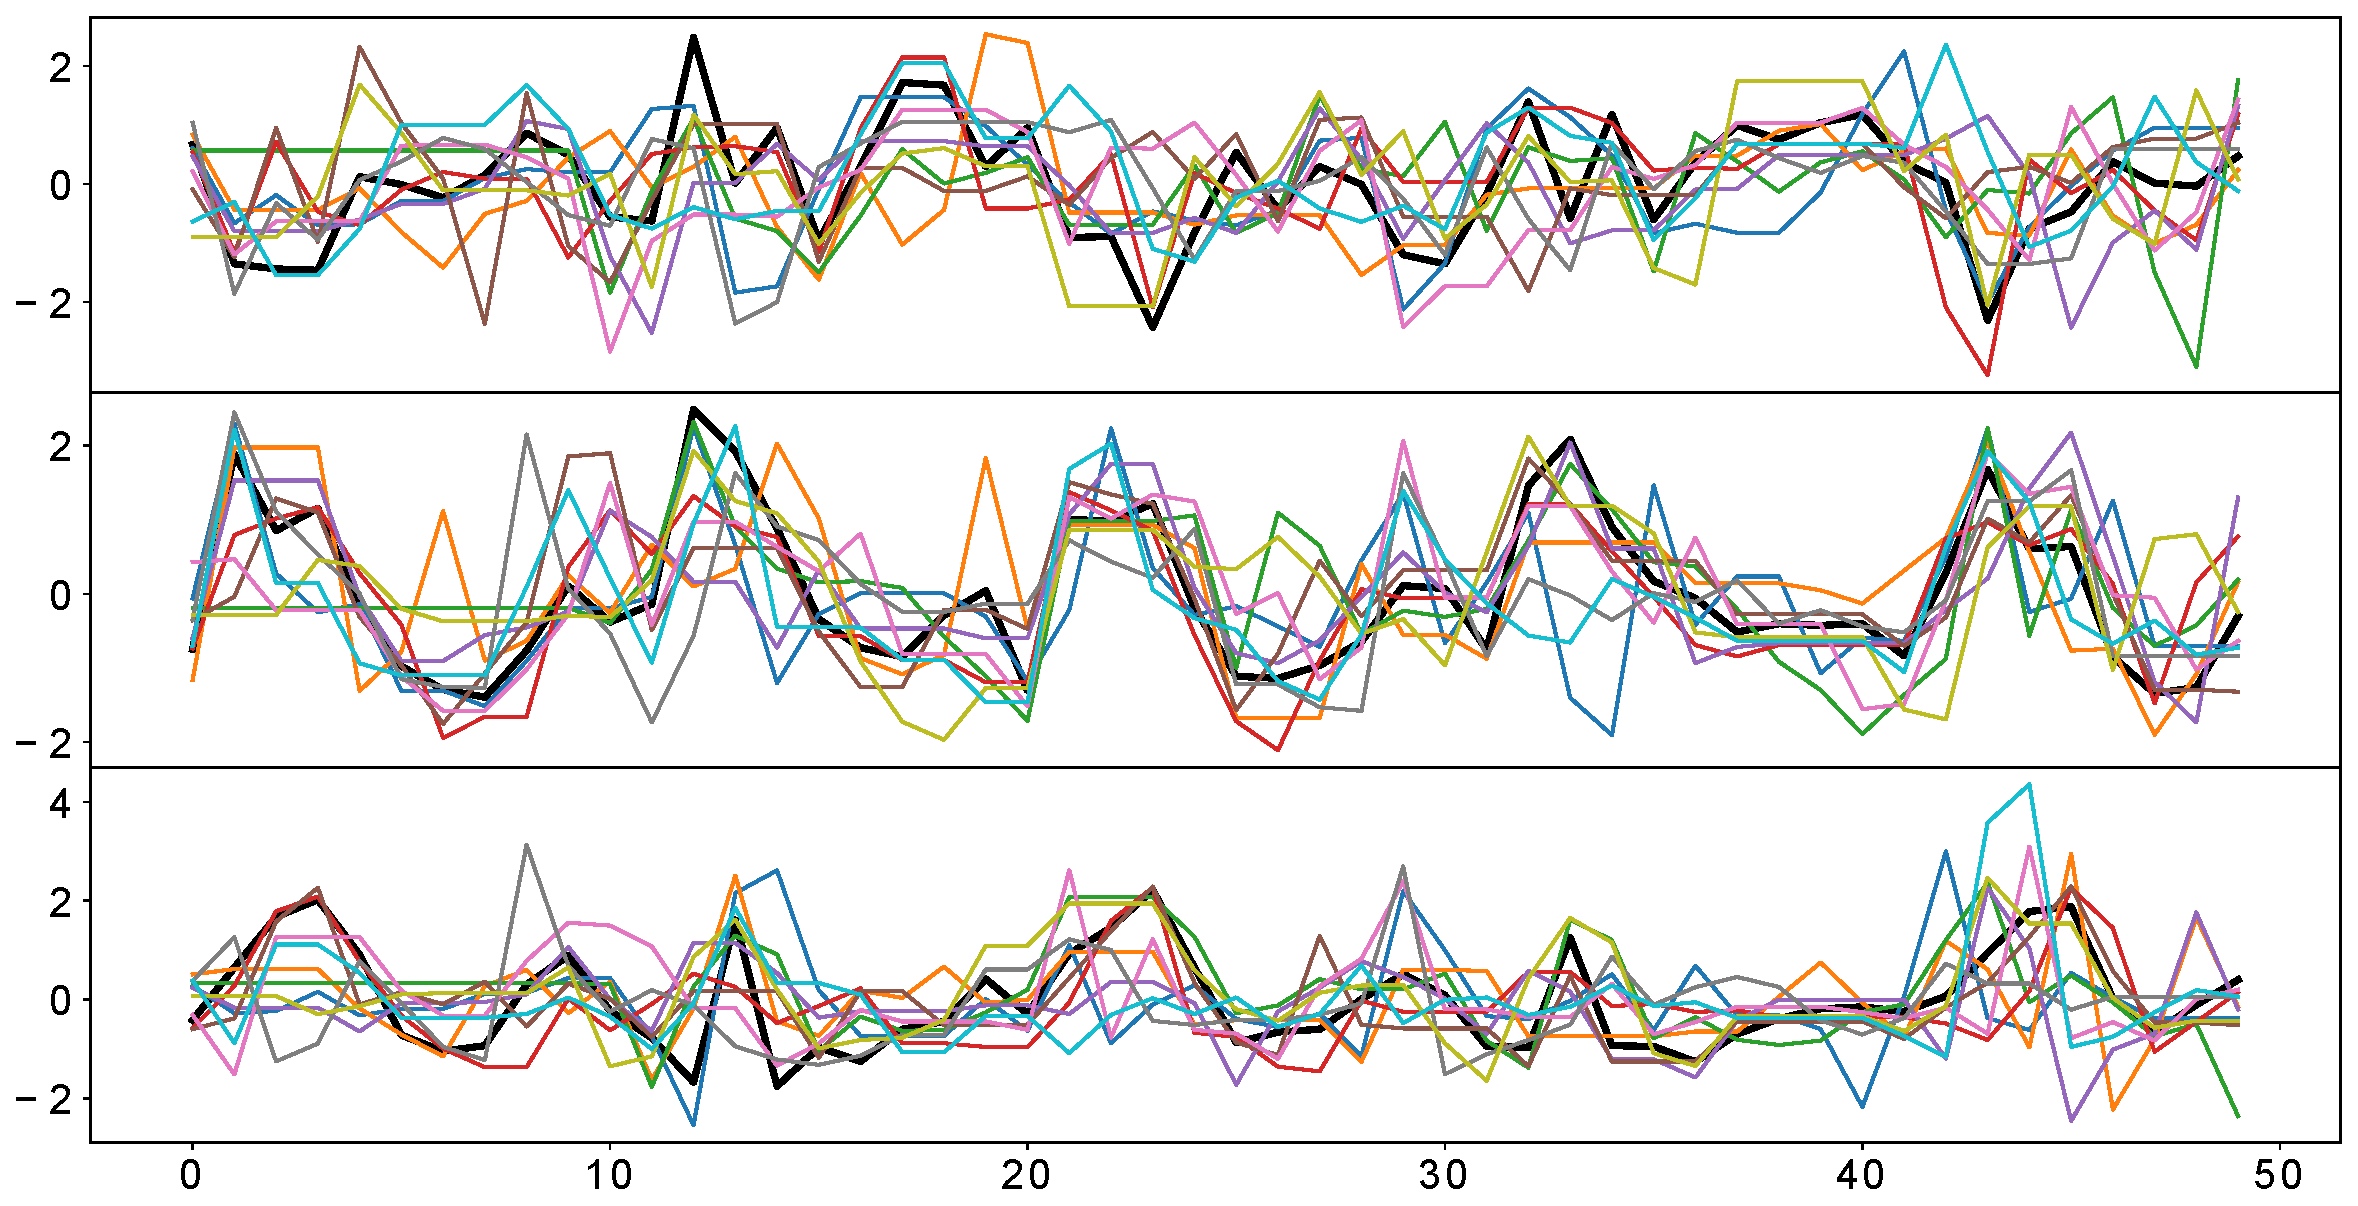
\includegraphics[width=\textwidth]{images/img3.eps}
        \caption{Кластеризация с $L_2$} \label{img2}
    \end{figure}                
    % \section{Заключение}
    
    

    \bibliography{literature} 
    \bibliographystyle{unsrt}
    
    % Решение Программного Комитета:
    %\ACCEPTNOTE
    %\AMENDNOTE
    %\REJECTNOTE
\end{document}
    

    
